\documentclass[tikz,border=14pt]{standalone}
\usepackage{tikz}
\usepackage{amsmath,amssymb}
\usetikzlibrary{arrows.meta, backgrounds, calc, fit}

% ── Palette ──────────────────────────────────────────────────────────
\definecolor{Csig} {RGB}{180,  30,  30}  % vibrant red
\definecolor{Cexp} {RGB}{ 60,  60, 180}  % vibrant indigo/blue
\definecolor{Cout} {RGB}{  0,  70,  80}  % high-contrast dark teal
\definecolor{Cbg}  {RGB}{255, 255, 255}  % pure white

\tikzset{
  N/.style    = {draw, fill=Cbg, align=center,
                 font=\small, line width=0.65pt, minimum height=0.95cm},
  Npath/.style= {N, minimum width=6.2cm, fill=white},
  Ng/.style   = {N, minimum width=6.2cm, fill=white},
  Nsig/.style = {N, minimum width=5.6cm, draw=Csig, text=Csig!80!black,  fill=Csig!6},
  Nexp/.style = {N, minimum width=5.6cm, draw=Cexp, text=Cexp!80!black,  fill=Cexp!6},
  Nout/.style = {N, minimum width=5.6cm, draw=Cout, text=Cout!80!black,  fill=Cout!7},
  Nopt/.style = {N, minimum width=6.2cm, minimum height=1.1cm,
                 draw=Cout, text=Cout!80!black, fill=Cout!9},
  Asig/.style = {-{Stealth[length=5pt,width=4pt]},  line width=0.70pt, color=Csig},
  Aexp/.style = {-{Stealth[length=5pt,width=4pt]},  line width=0.70pt, color=Cexp},
  Apath/.style= {-{Stealth[length=5pt,width=4pt]},  line width=0.70pt},
  Ag/.style   = {-{Stealth[length=5pt,width=4pt]},  line width=0.70pt},
  Lbl/.style  = {font=\small\itshape, text=gray!55!black},
  Brh/.style  = {font=\small\bfseries,
                 inner sep=4pt, fill=white, draw=gray!35},
}

\begin{document}
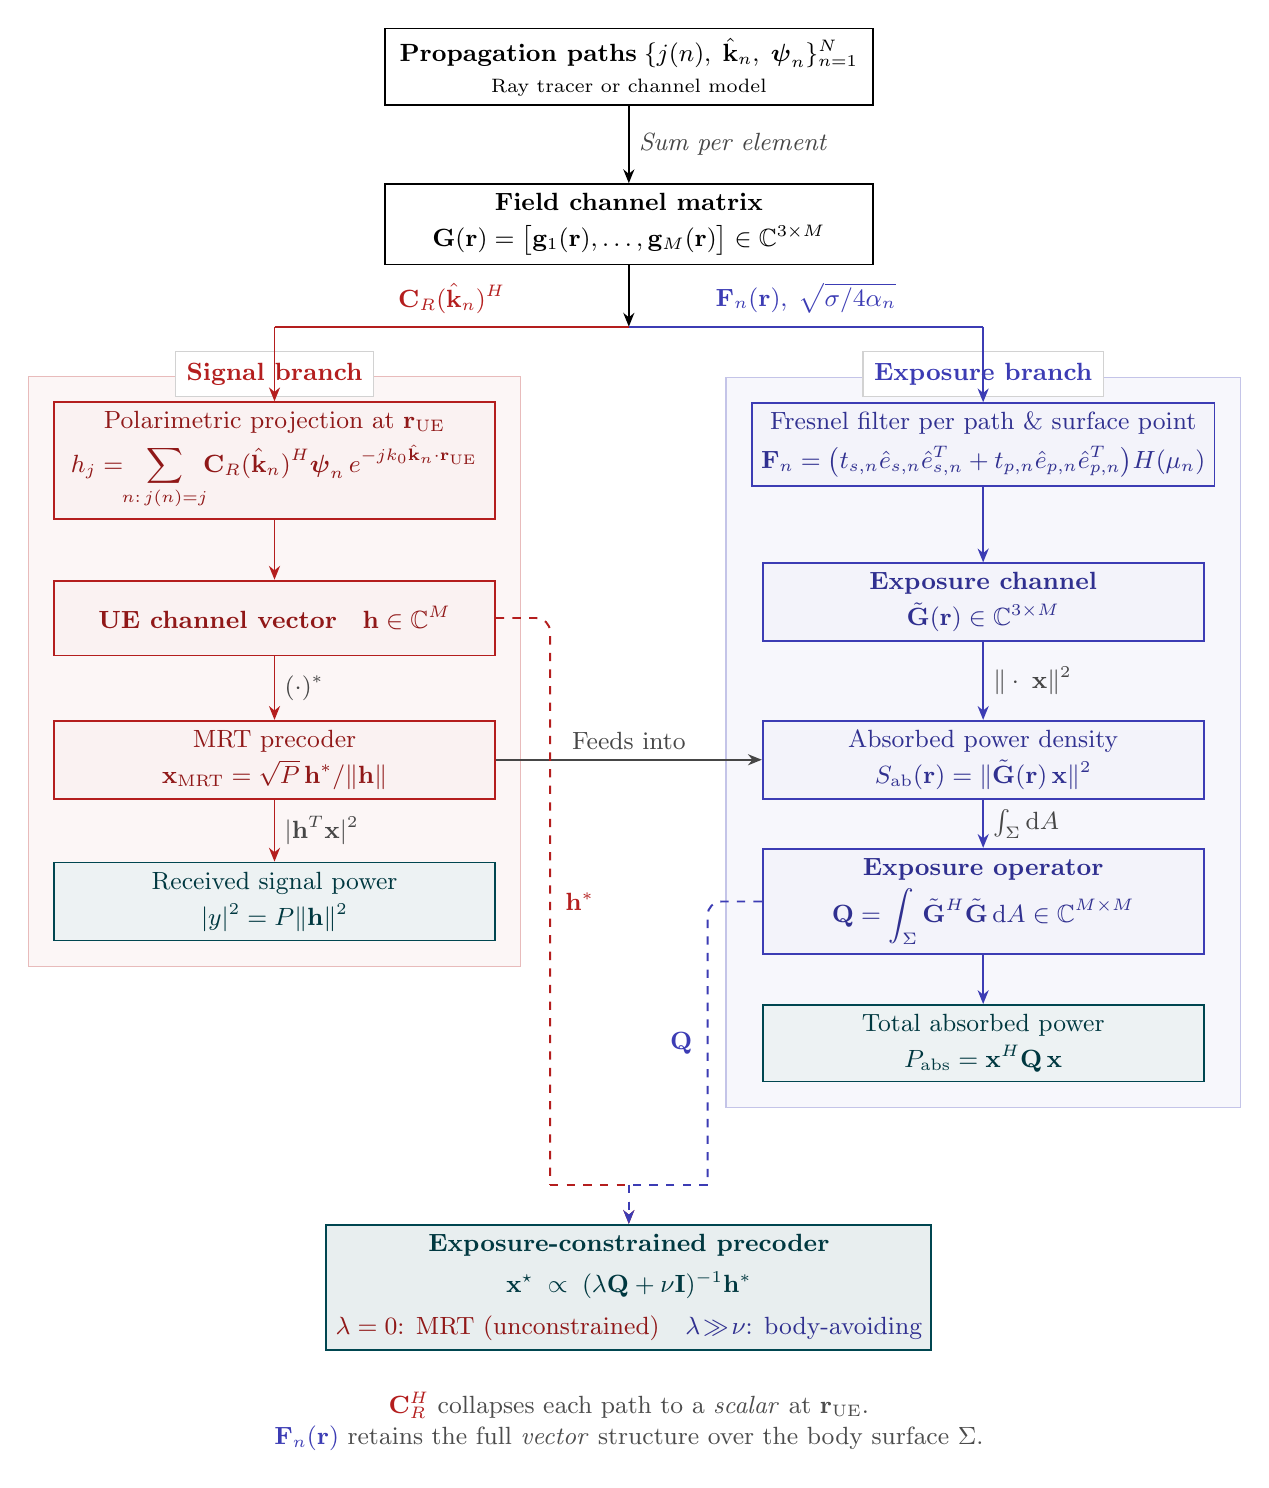
\begin{tikzpicture}

%% ─────────────────────────────────────────────────────────────────────
%%  COLUMN X POSITIONS
%%  Centre: 0   |   Signal: -4.5   |   Exposure: +4.5
%% ─────────────────────────────────────────────────────────────────────

% TOP: propagation paths  (centre column, y=0)
\node[Npath] at (0, 0)       (paths)
  {\textbf{Propagation paths}\;$\{j(n),\;\hat{\mathbf{k}}_n,\;\boldsymbol{\psi}_n\}_{n=1}^N$\\
   {\scriptsize Ray tracer or channel model}};

% Field channel G(r)   (y = -2.0)
\node[Ng]    at (0, -2.0)    (Gr)
  {\textbf{Field channel matrix}\\[2pt]
   $\mathbf{G}(\mathbf{r})=\bigl[\mathbf{g}_1(\mathbf{r}),\ldots,\mathbf{g}_M(\mathbf{r})\bigr]
   \in\mathbb{C}^{3\times M}$};

%% ── Bus fork at y = -3.3 ──
\coordinate (busC) at (0,     -3.3);
\coordinate (busL) at (-4.5,  -3.3);
\coordinate (busR) at ( 4.5,  -3.3);


%% ── Branch labels at y = -3.8 (well above first column boxes) ──
\node[Brh, text=Csig] at (-4.5, -3.9) {Signal branch};
\node[Brh, text=Cexp] at ( 4.5, -3.9) {Exposure branch};

%% ── Signal column  (x = -4.5) ── y steps: 5.0, 7.0, 8.8, 10.6
\node[Nsig]  at (-4.5, -5.0) (hdef)
  {Polarimetric projection at $\mathbf{r}_\text{UE}$\\[3pt]
   $h_j =\!\!\displaystyle\sum_{n:\,j(n)=j}\!\!
     \mathbf{C}_R(\hat{\mathbf{k}}_n)^H\boldsymbol{\psi}_n\,
     e^{-jk_0\hat{\mathbf{k}}_n\cdot\mathbf{r}_\text{UE}}$};

\node[Nsig]  at (-4.5, -7.0) (hvec)
  {\textbf{UE channel vector}\quad $\mathbf{h}\in\mathbb{C}^M$};

\node[Nsig]  at (-4.5, -8.8) (mrt)
  {MRT precoder\\[2pt]$\mathbf{x}_\text{MRT}=\sqrt{P}\,\mathbf{h}^*/\|\mathbf{h}\|$};

\node[Nout]  at (-4.5, -10.6) (sigout)
  {Received signal power\\[2pt]$|y|^2 = P\|\mathbf{h}\|^2$};

%% ── Exposure column  (x = +4.5) ── shifted up 0.2 cm to align panel top with signal
\node[Nexp]  at (4.5, -4.8)  (fresnel)
  {Fresnel filter per path \& surface point\\[3pt]
   $\mathbf{F}_n = \bigl(t_{s,n}\hat{e}_{s,n}\hat{e}_{s,n}^T
                 + t_{p,n}\hat{e}_{p,n}\hat{e}_{p,n}^T\bigr)H(\mu_n)$};

\node[Nexp]  at (4.5, -6.8)  (Gtilde)
  {\textbf{Exposure channel}\\[2pt]$\tilde{\mathbf{G}}(\mathbf{r})\in\mathbb{C}^{3\times M}$};

\node[Nexp]  at (4.5, -8.8)  (Sab)
  {Absorbed power density\\[2pt]$S_\text{ab}(\mathbf{r}) = \|\tilde{\mathbf{G}}(\mathbf{r})\,\mathbf{x}\|^2$};

\node[Nexp]  at (4.5, -10.6)  (Qop)
  {\textbf{Exposure operator}\\[2pt]
   $\mathbf{Q}=\displaystyle\int_\Sigma\tilde{\mathbf{G}}^H\tilde{\mathbf{G}}\,\mathrm{d}A
               \in\mathbb{C}^{M\times M}$};

\node[Nout]  at (4.5, -12.4) (Pabs)
  {Total absorbed power\\[2pt]$P_\text{abs}=\mathbf{x}^H\mathbf{Q}\,\mathbf{x}$};

%% ── Constrained precoder  (centre, y = -15.5)
\node[Nopt]  at (0, -15.5)   (opt)
  {\textbf{Exposure-constrained precoder}\\[4pt]
   $\mathbf{x}^\star \;\propto\; (\lambda\mathbf{Q}+\nu\mathbf{I})^{-1}\mathbf{h}^*$\\[4pt]
   \textcolor{Csig!80!black}{$\lambda=0$: MRT (unconstrained)}\quad
   \textcolor{Cexp!80!black}{$\lambda\!\gg\!\nu$: body-avoiding}};

%% ─────────────────────────────────────────────────────────────────────
%%  ARROWS — top to field channel
%% ─────────────────────────────────────────────────────────────────────
\draw[Apath] (paths) -- node[right,Lbl]{Sum per element} (Gr);

%% ─────────────────────────────────────────────────────────────────────
%%  FORK: G(r).south → bus → each column
%% ─────────────────────────────────────────────────────────────────────
%% green down-stroke from G(r) to bus
\draw[Ag] (Gr.south) -- (busC);

%% red fork left → signal column  (no arrowhead on horizontal bus leg)
\draw[Asig, -] (busC) -- (busL)
  node[midway, above, Lbl, text=Csig, yshift=1pt]{$\mathbf{C}_R(\hat{\mathbf{k}}_n)^H$};
\draw[Asig] (busL) -- (hdef.north);

%% purple fork right → exposure column  (no arrowhead on horizontal bus leg)
\draw[Aexp, -] (busC) -- (busR)
  node[midway, above, Lbl, text=Cexp, yshift=1pt]{$\mathbf{F}_n(\mathbf{r}),\;\sqrt{\sigma/4\alpha_n}$};
\draw[Aexp] (busR) -- (fresnel.north);

%% ─────────────────────────────────────────────────────────────────────
%%  SIGNAL branch internal
%% ─────────────────────────────────────────────────────────────────────
\draw[Asig] (hdef)  -- (hvec);
\draw[Asig] (hvec)  -- node[right,Lbl]{$(\cdot)^*$}                  (mrt);
\draw[Asig] (mrt)   -- node[right,Lbl]{$|\mathbf{h}^T\mathbf{x}|^2$} (sigout);

%% Cross-branch: mrt.east → Sab  (feeds into)
\draw[-{Stealth[length=5pt,width=4pt]}, line width=0.70pt, color=gray!55!black]
  (mrt.east) -- node[above, font=\small, text=gray!55!black]{Feeds into} (Sab.west);

%% ─────────────────────────────────────────────────────────────────────
%%  EXPOSURE branch internal
%% ─────────────────────────────────────────────────────────────────────
\draw[Aexp] (fresnel) -- (Gtilde);
\draw[Aexp] (Gtilde)  -- node[right,Lbl]{$\|\cdot\;\mathbf{x}\|^2$}  (Sab);
\draw[Aexp] (Sab)     -- node[right,Lbl]{$\int_\Sigma \mathrm{d}A$}            (Qop);
\draw[Aexp] (Qop)     -- (Pabs);

%% ─────────────────────────────────────────────────────────────────────
%%  DASHED MERGE ARROWS
%%  Both cross to centre lane x=0 at y=-14.2, then drop due-south into
%%  opt.north  →  arrowhead always points south, no diagonal segments.
%% ─────────────────────────────────────────────────────────────────────

%% Named waypoints
\coordinate (hLane) at (-1.0, -7.0);   %% signal: turn into centre gap
\coordinate (hBend) at (-1.0, -14.2);  %% signal: bottom of vertical lane
\coordinate (qLane) at ( 1.0, -10.6);  %% exposure: turn into centre gap
\coordinate (qBend) at ( 1.0, -14.2);  %% exposure: bottom of vertical lane
\coordinate (cTop)  at (0,   -14.2);   %% shared centre entry, above opt.north

%% Signal: hvec.east → right → down (labelled h*) → centre → opt.north
\draw[Asig, dashed, -, rounded corners=5pt]
  (hvec.east) -- (hLane) -- (hBend);
\path (hLane) -- (hBend)
  node[midway, right, Lbl, text=Csig, xshift=2pt]{$\mathbf{h}^*$};
\draw[Asig, dashed, -]  (hBend) -- (cTop);
\draw[Asig, dashed]     (cTop)  -- (opt.north);

%% Exposure: Qop.west → left → down (labelled Q) → centre → opt.north
\draw[Aexp, dashed, -, rounded corners=5pt]
  (Qop.west) -- (qLane) -- (qBend);
\path (qLane) -- (qBend)
  node[midway, left, Lbl, text=Cexp, xshift=-2pt]{$\mathbf{Q}$};
\draw[Aexp, dashed, -]  (qBend) -- (cTop);
\draw[Aexp, dashed]     (cTop)  -- (opt.north);

%% ─────────────────────────────────────────────────────────────────────
%%  CAPTION
%% ─────────────────────────────────────────────────────────────────────
\node[font=\small, text=gray!60!black, align=center]
  at (0, -17.2)
  {\textcolor{Csig}{$\mathbf{C}_R^H$} collapses each path to a \emph{scalar} at $\mathbf{r}_\text{UE}$.\\
   \textcolor{Cexp}{$\mathbf{F}_n(\mathbf{r})$} retains the full \emph{vector} structure over the body surface $\Sigma$.};

%% ─────────────────────────────────────────────────────────────────────
%%  BACKGROUND PANELS
%% ─────────────────────────────────────────────────────────────────────
\begin{scope}[on background layer]
  \node[fit=(hdef)(hvec)(mrt)(sigout),
        draw=Csig!30, fill=Csig!4, inner sep=9pt] {};
  \node[fit=(fresnel)(Gtilde)(Sab)(Qop)(Pabs),
        draw=Cexp!30, fill=Cexp!4, inner sep=9pt] {};
\end{scope}

\end{tikzpicture}
\end{document}
